\documentclass[twoside,11pt]{article}

% Any additional packages needed should be included after jmlr2e.
% Note that jmlr2e.sty includes epsfig, amssymb, natbib and graphicx,
% and defines many common macros, such as 'proof' and 'example'.
%
% It also sets the bibliographystyle to plainnat; for more information on
% natbib citation styles, see the natbib documentation, a copy of which
% is archived at http://www.jmlr.org/format/natbib.pdf

\usepackage{jmlr2e}
%\usepackage{parskip}

% Definitions of handy macros can go here
\newcommand{\dataset}{{\cal D}}
\newcommand{\fracpartial}[2]{\frac{\partial #1}{\partial  #2}}
% Heading arguments are {volume}{year}{pages}{submitted}{published}{author-full-names}

% Short headings should be running head and authors last names
\ShortHeadings{95-845: AAMLP FINAL PROJECT}{MICHELLE AND YA-TING}
\firstpageno{1}
\usepackage{subcaption}
\usepackage[square,numbers]{natbib}
\bibliographystyle{unsrtnat}


\begin{document}

%\title{Heinz 95-845: Article Title on \\ Applied Analytics: the Machine Learning Pipeline}
\title{Prediction of Septic Shock for ICU patients \\with Chronic Diseases}

\author{\name Michelle Hus \email mhsu1@andrew.cmu.edu \\
       \addr Heinz College\\
       Carnegie Mellon University\\
       Pittsburgh, PA, United States
       \AND
       \name Ya-Ting Chang \email yatingc2@andrew.cmu.edu\\
       \addr Heinz College\\
       Carnegie Mellon University\\
       Pittsburgh, PA, United States}

\maketitle

\begin{abstract}
	We predicted the probability of onset of sepsis, severe sepsis and septic shock for patient in Intensive Care Unit (ICU). The 1,640 subjects are selected from the public database MIMIC-II.  Specifically, the population of this study is patients with diabetes, kidney and lung related chronic disease. We used ensembling machine learning methods to predict outcome, and compared different algorithms for sepsis prediction. 
\end{abstract}
\section{Introduction}
Sepsis is the body's extreme response to an infection. It is defined as a combination of Systemic Inflammatory Response Syndrome (SIRS), and a confirmed or suspected infection, usually caused by bacteria\cite{cite2}. Untreated or inadequately treated cases of sepsis can lead to condition known as severe sepsis or septic shock. Septic shock is defined as a subset of sepsis in which particularly profound circulatory, cellular, and metabolic abnormalities are associated with a greater risk of mortality than with sepsis alone. Therefore, early diagnosis of sepsis is essential for successful treatment.

In adults, Systemic Inflammatory Response Syndrome (SIRS) is defined as the presence of two or more of the following\cite{cite1}:
\begin{enumerate}
	\item Body temperature below 36°C (96.8°F) or above 38°C (100.4°F) 
	\item Tachycardia, with heart rate above 90 beats per minute
	\item Tachypea (increased respiratory rate), with respiratory rate above 20 per minute
	\item White blood cell (WBC) count less than 4,000/mm3(cubic millimeter) or above 12,000/mm3
\end{enumerate}

Many automated sepsis screening tools described in the literature are primarily based on SIRS criteria, with additional specifications that are tailored to individual hospital systems\cite{cite3}. A recently developed risk stratification tool that was presented along with the new sepsis definitions is termed the quick sepsis-related organ failure assessment (qSOFA). It uses three criteria, assigning one point for low blood pressure (SBP $<$ 100 mmHg), high respiratory rate ($\geq$ breaths per min), or altered mentation (Glasgow coma scale $<$ 15). The score ranges from 0 to 3 points. The presence of 2 or more qSOFA points near the onset of infection was associated with a greater risk of death or prolonged intensive care unit stay. 

Recent advances in early detection of sepsis have resulted in substantial progress in predicting the onset of sepsis for ICU patients. 
However, many studies focus on the general ICU patient without considering their medical histories. According to Centers for Disease Control and Prevention, though anyone can get an infection, certain people are at higher risk: 
\begin{itemize}
	\item Adults 65 or older
	\item People with chronic medical conditions, such as diabetes, lung disease, cancer, and kidney disease
	\item People with weakened immune systems
	\item Children younger than one
\end{itemize}

Our goal was to detect the presence of sepsis for ICU patient with chronic diseases such as diabetes, lung disease and kidney disease. By identifying patients with these medical conditions, we hope to provide a powerful prediction for the risk of sepsis, severe sepsis, and septic shock so that hospitals can better initiate prevention strategies for these patients.



\section{Experimental Setup}
\begin{figure}[!htbp]
	\centering 
	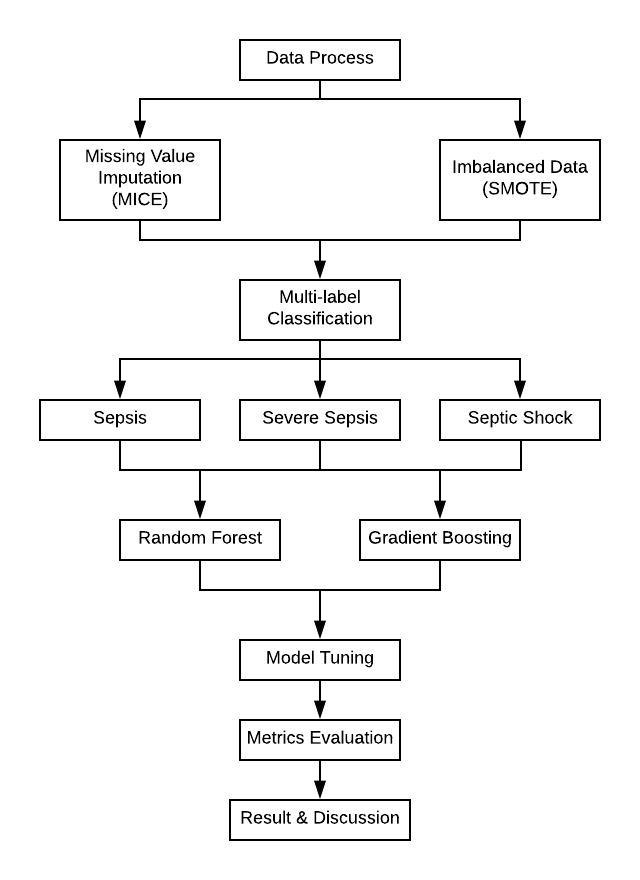
\includegraphics[width=4in]{Pipeline.jpeg} 
	\caption{Pipeline}
	\label{fig:example} 
\end{figure} 
\subsection{Cohort Selection}
The dataset used in this study is from MIMIC II (Multiparameter Intelligent Monitoring in Intensive Care), which is the clinical data collected from Beth Israel Deaconess Medical Center.
Since our study focuses on patients with chronic diseases, the cohort is comprised of ICU patients with diabetes, chronic kidney diseases, and chronic lung diseases.

\begin{table}[htbp]
	\centering 
	\begin{tabular}{|p{4cm}|p{2cm}|p{2cm}|p{2cm}|}
		\hline 
		& Diabetes(\%) & Kidney(\%) & Lung(\%)\\ 
		\hline \\[-11pt]
		Sepsis (n=40) & 80 &  25 & 15 \\ 
		Severe Sepsis (n=217) & 73.3 &  29.9 & 10.1\\
		Septic Shock (n=109) & 72.5 & 24.8 & 11.9\\
		\hline 
	\end{tabular}
	\label{tab:example} 
	\caption{Chronic Disease(\%) for each Syndrome} 
\end{table}

\begin{table}[htbp]
	\centering 
	\begin{tabular}{lclc} 
		& Mean & Median \\ 
		\hline \\[-11pt]
		Blood Pressure & 76.01 & 74.87 \\ 
		Heart Rate & 85.18 & 84.02\\
		Respiratory Rate & 19.98 & 19.52\\
		Oxygen Saturation & 96.75 & 97.24\\
		Temperature & 98.05 & 98.10\\
		\hline 
	\end{tabular}
	\label{tab:example} 
	\caption{Vital Signs Statistics of Chronic Disease Patients (n=1,640)} 
\end{table}

\subsection{Data Extraction}
Extracted from the MIMIC II dataset, we utilized the tables containing hospitalization information, vital signs measurement, patient demographics, and medical diagnosis. Regarding the data preprocessing, we first identify the code of our interested chronic diseases (diabetes, kidney, and lung) and the targets (sepsis, severe sepsis, and septic shock). We then filter the hospitalization (hadm\_id) with the identified chronic disease. For these selected hospitalizations, we used one-hot encoding to transform the three diseases into the binary representation. As for the outcome variables, we also conducted the binary transformation and joined the two wide-format tables using column "hadm\_id", resulting in a table with each row representing a unique hospitalization. For the next step, we added other features such as the vital signs and demographic information to the wide-format table by hadm\_id. In the original data from MIMIC II, each instance represents a unique ICU stay. Therefore, one hospitalization can have several records of the same vital sign since a patient can be admitted to ICU more than one time per hospitalization. To address the multiple records issue, we averaged the vital sign measurements among the ICU stays to represent the unique hospitalization. After the data preprocessing, the final table contains 1,640 rows with 20 features. For our analysis, we assumed each hospitalization is independent and treated each hospitalization as one instance.

Before running the model, we handled the problems of missing values and imbalanced data in our dataset. Regarding the missing values, the issue primarily comes from the vital sign features with blood pressure containing the highest percentage (7.99\%) of missing values. We adopted MICE (Multivariate Imputation by Chained Equations) as our imputation method with the assumption that the values are missing at random. As for the imbalanced data, we implemented SMOTE (Synthetic Minority Over-Sampling Technique) to overcome the skewed dataset. SMOTE incorporates the k nearest neighbor as the underlying method to over-sample the minority class and under-sample the majority class. 

\begin{table}[htbp]
	\centering 
	\begin{tabular}{lclc}
		\hline 
		& Missing Value(\%) \\ 
		\hline \\[-11pt]
		Sex & 0.366\\ 
		Age & 0.122\\
		Blood Pressure & 7.99\\
		Heart Rate & 4.82\\
		Respiratory Rate & 5.06\\
		Oxygen Rate & 5.06\\
		Temperature & 6.52\\
		\hline 
	\end{tabular}
	\label{tab:missing} 
	\caption{Missing value(\%) of predictors} 
\end{table}

\begin{table}[htbp]
	\centering 
	\begin{tabular}{|p{3cm}|p{3cm}|p{3cm}|p{3cm}|}
		\hline 
		& Sepsis(\%) & Severe Sepsis(\%) & Septic Shock(\%)\\ 
		\hline \\[-11pt]
		Original & 2.44 &  13.2 & 6.65 \\ 
		SMOTE & 26.8 &  42.9 & 27.6\\
		\hline 
	\end{tabular}
	\label{tab:imbalance} 
	\caption{Imbalanced data(\%) with SMOTE} 
\end{table}

\subsection{Feature Choices}
The features in this study is composed of 4 categories: demographics, vital signs, chronic disease indicator, and the outcome variables. The original variables including race and diagnosis were converted to dummy variables with the binary representation since we want to assess the importance of each variable in terms of the 3 syndromes. To implement random forest and gradient boosting algorithms, we then transformed the outcome variables (sepsis, severe sepsis, and septic shock) into categorical variables. 

\begin{table}[htbp]
	\centering 
	\begin{tabular}{|p{2.7cm}|p{13cm}|}
		\hline 
		& Feature\\ 
		\hline \\[-11pt]
		Demographic &  age, sex, white, asian, black, hispanic, others, unknown\\ 
		Vital Signs & blood.pressure, heart.rate, respiratory.rate, oxygen.saturation, temperature\\
		Chronic Disease & diabetes, kidney, lung\\
		Outcome & Sepsis, SeverSepsis, SepticShock\\
		\hline 
	\end{tabular}
	\label{tab:example} 
	\caption{Feature Selection} 
\end{table}

\subsection{Comparison Methods}
Our analysis used the similar approach with the study from BMJ Journal\cite{cite6}, which implemented ensemble machine learning techniques to evaluated the existing sepsis prediction algorithm (InSight). Compared to the study which adopted 10-fold cross validation on gradient boosting method to predict the onset of sepsis, severe sepsis, and septic shock, we used only 5-fold cross validation yet incorporated the tuning process on the max depth of each tree and the number of boosting iterations. 
\subsection{Evaluation Criteria}
Besides the accuracy rate, we assessed our models with ROC curve and AUC to ensure the result is not biased by the skewness of the dataset even though we handled the imbalanced data using SMOTE in the earlier step. 

\section{Method: Gradient Boosting and Random Forest} \label{model}
Since sepsis, severe sepsis and septic shock could happen sequentially to a patient in a single hospitalization, our task is a multi-label classification task. Our approach is to take binary relevance method, independently training one binary classifier for each label. 

We choose Naive Bayes method as our baseline, and use two ensemble learning methods as our classifiers: random forest and gradient boosting method. The reason we chose these algorithms is that we believe that the accuracy of our prediction is of great significance. Compared to decision tree whose advantage is its interpretability, and logistic regression whose advantage is that it could also inform us the coefficients of features, we put more emphasis on the accuracy. 

For each syndrome, we fit gradient boosting and random forest models, tuned the hyperparameters of each models, predicted the test data with optimal parameters chosen through cross-validation. 

\subsection{Gradient Boosting}
For gradient boosting, we tuned two hyperparameters: number of boosting iterations and maximum of tree depth. For example, after cross validation for the sepsis prediction, we found that the optimal number of iteration is 3,600 and optimal tree depth is 15, given the shrinkage rate is 0.001 and minimum terminated node size is 30.

\subsection{Random Forest}
For random forest, we tuned two hyperparameters: number of trees and number of nodes at each split.
The node impurity is measured by Gini index. In the result section, we also presented the variable importance for the prediction.  


\section{Results} \label{results}
Resulted are presented by comparing two different algorithms for each syndromes (Sepsis, severe sepsis,septic shock). 

\subsection{Results on Sepsis} 
Gradient Boosting outperforms the other two methods in terms of AUC and accuracy rate.
\begin{table}[htbp]
  \centering 
  \begin{tabular}{lclc} 
    Method & Accuracy(\%) & AUC(\%) \\ 
    \hline \\[-11pt]
    Naive Bayes & 78 & 84 \\ 
    Random Forest & 77 & 84 \\ 
    Gradient Boosting & 89 & 93 \\ \hline 
  \end{tabular}
  \label{tab:outcome} 
    \caption{Sepsis Prediction Outcome} 
\end{table}

\begin{figure}[htbp]
\begin{subfigure}{.5\textwidth}
	\centering 
	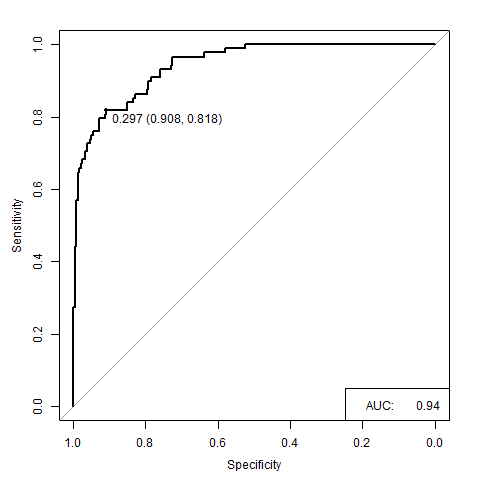
\includegraphics[width=2.5in]{gbm_sepsis_auc.png} 
	\caption{Gradient Boosting}
	\label{fig:gbm_sepsis} 
\end{subfigure}%
\begin{subfigure}{.5\textwidth}
	\centering 
	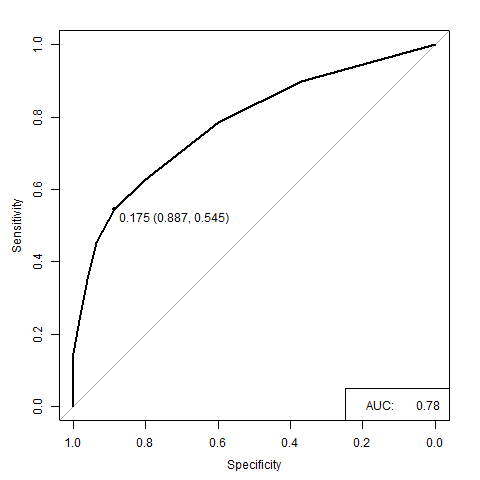
\includegraphics[width=2.5in]{rf_sepsis_auc.png} 
	\caption{Random Forest}
	\label{fig:rf_sepsis} 
\end{subfigure}
\caption{ROC curve}
\label{fig:fig}
\end{figure}  

\begin{figure}[htbp]
	\centering
	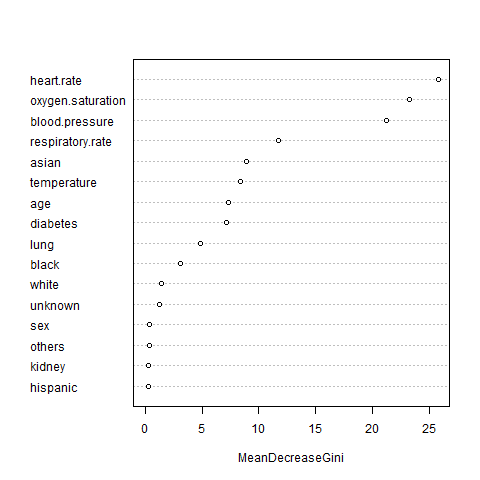
\includegraphics[width=3.5in]{rf_var_sepsis.png} 
	\caption{Variable Importance}
	\label{fig:var}
\end{figure}

\subsection{Results on Severe Sepsis}
Same results apply to severe sepsis and septic shock.
(see page 8)
\begin{table}[htbp]
 	\centering 
 	\begin{tabular}{lclc} 
 		Method & Accuracy(\%) & AUC(\%) \\ 
 		\hline \\[-11pt]
 		Naive Bayes & 68 & 72 \\ 
 		Random Forest & 73 & 83 \\ 
 		Gradient Boosting & 80 & 88 \\ \hline 
 	\end{tabular}
 	\label{tab:outcome} 
 	\caption{Severe Sepsis Prediction Outcome} 
\end{table}
\begin{figure}[htbp]
 	\begin{subfigure}{.5\textwidth}
 		\centering 
 		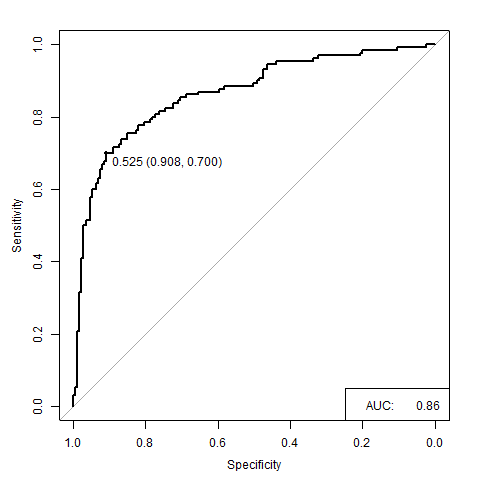
\includegraphics[width=3in]{gbm_severe_auc.png} 
 		\caption{Gradient Boosting}
 		\label{fig:gbm_severe} 
 	\end{subfigure}%
 	\begin{subfigure}{.5\textwidth}
 		\centering 
 		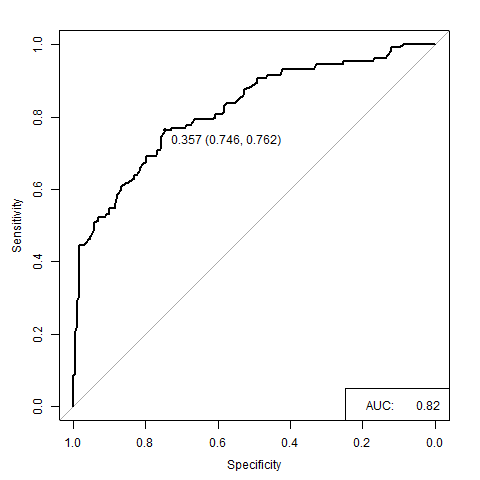
\includegraphics[width=3in]{rf_severe_auc.png} 
 		\caption{Random Forest}
 		\label{fig:rf_severe} 
 	\end{subfigure}
 	\caption{ROC curve}
 	\label{fig:fig}
\end{figure} 

\begin{figure}[htbp]
	\centering
	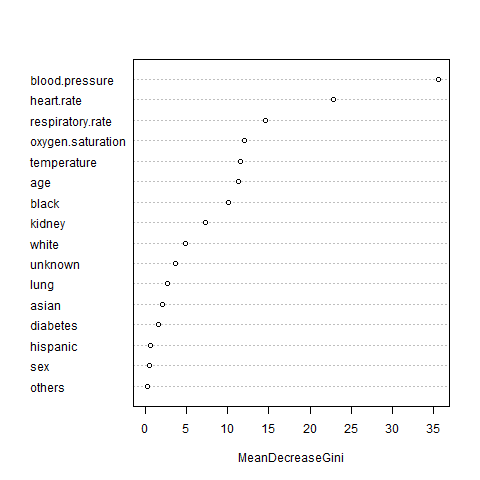
\includegraphics[width=3.5in]{rf_var_severe.png} 
	\caption{Variable Importance}
	\label{fig:var}
\end{figure} 


\subsection{Results on Septic Shock}
(see page 9)
\begin{table}[htbp]
	\centering 
	\begin{tabular}{lclc} 
		Method & Accuracy(\%) & AUC(\%) \\ 
		\hline \\[-11pt]
		Naive Bayes & 82 & 80 \\ 
		Random Forest & 82 & 85 \\ 
		Gradient Boosting & 89 & 91 \\ \hline 
	\end{tabular}
	\label{tab:outcome} 
	\caption{Septic Shock Prediction Outcome} 
\end{table}

\begin{figure}[htbp]
	\begin{subfigure}{.5\textwidth}
		\centering 
		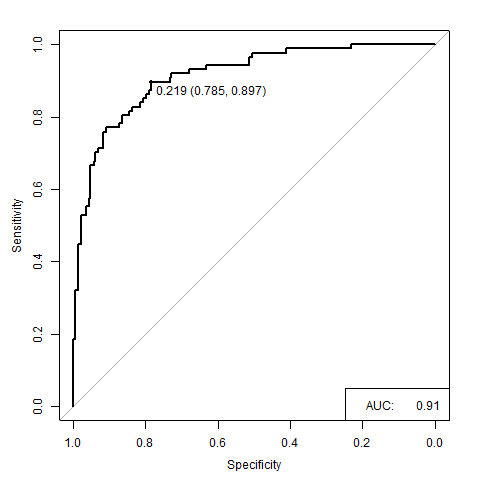
\includegraphics[width=3in]{gbm_shock_auc.png} 
		\caption{Gradient Boosting}
		\label{fig:gbm_shock} 
	\end{subfigure}%
	\begin{subfigure}{.5\textwidth}
		\centering 
		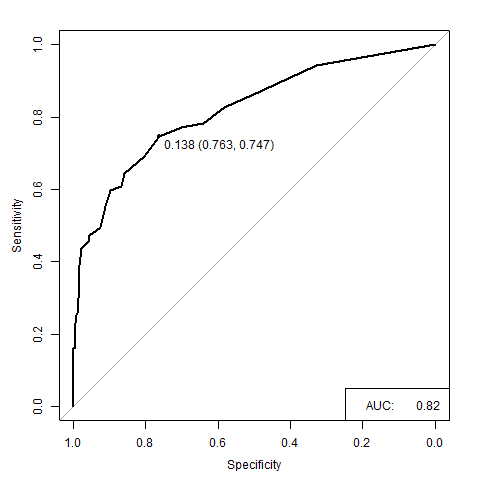
\includegraphics[width=3in]{rf_shock_auc.png} 
		\caption{Random Forest}
		\label{fig:rf_shock} 
	\end{subfigure}
	\caption{ROC curve}
	\label{fig:fig}
\end{figure}  

\begin{figure}[htbp]
	\centering
	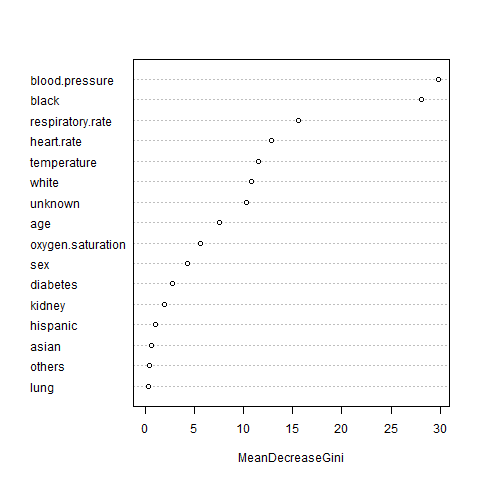
\includegraphics[width=3.5in]{rf_var_shock.png} 
	\caption{Variable Importance}
	\label{fig:var}
\end{figure} 

\section{Discussion and Related Work} 
Based on the result of our study, we can conclude that vital signs are important indicators for predicting the onset of sepsis, severe sepsis, and septic shock, which is in line with the findings from the paper by BMJ Journal\cite{cite6}. Also, for different levels of sepsis condition, certain race exhibits different level of importance for the prediction. For instance, race black is an important variable while predicting septic shock. Therefore, by taking race into consideration, doctors can be more informed of the risk of sepsis condition for the patients with chronic diseases. However, there are some limitations for the study. We only focused on the ICU patients with certain type of chronic diseases (diabetes, kidney diseases, and lung disease). Hence, the result only applies to patients with the specific medical condition. The other limitation is derived from the small sample size of the analysis. Our models were constructed upon 1,640 instances, which may generate different results with larger sample size. In addition, MIMIC II is not the most updated dataset. The clinical data only ranges from 2001 to 2008. To generalize our study, we will need to use a more recent dataset from MIMIC III.
\section{Conclusion} 
In sum, the study focuses on the prediction of the onset of sepsis-related condition for ICU patients with diabetes, chronic kidney disease, or chronic lung disease. We divided the original multi-label classification problem into 3 binary classification tasks and leveraged the ensemble machine learning method with Naïve Bayes as our baseline. For future extension on the study, we will include other types of chronic diseases such as cancer and cardiovascular disease. Additionally, using a more up-to-date database such as MIMIC III to analyze sepsis-related syndromes will also be our focus.

\bibliographystyle{plain}
\bibliography{sample}
\appendix
\end{document}
